\documentclass{beamer}
%\usetheme{Ilmenau}
%\usecolortheme{beaver}

\usepackage[slovak,american]{babel}
\usepackage[utf8]{inputenc}
\usepackage{graphicx}
\usepackage{adjustbox}
 \usepackage{xcolor}
 
 \newsavebox\MBox
\newcommand\Cline[2][red]{{\sbox\MBox{$#2$}%
  \rlap{\usebox\MBox}\color{#1}\rule[-2.2\dp\MBox]{\wd\MBox}{1pt}}}

%\usefonttheme{serif}

\definecolor{UKOrange}{HTML}{ef9424} %
\definecolor{UKBrown}{HTML}{a96d5e} %
\definecolor{UKLight}{HTML}{d8b6ab} %
\definecolor{UKDark}{HTML}{7a4f44}
\definecolor{UKDarker}{HTML}{4d312b} 
\definecolor{UKDarkest}{HTML}{2e1e1a}
\definecolor{UKRed}{HTML}{bf1f1c}

\setbeamertemplate{footline}[frame number]{}
\setbeamertemplate{navigation symbols}{}

%\usecolortheme{beaver}
\setbeamertemplate{itemize item}[square]
\setbeamercolor{itemize item}{fg = UKBrown}
\setbeamercolor{itemize subitem}{fg = UKLight}
\setbeamercolor{enumerate item}{fg = UKDark}

\setbeamercolor{footnote}{fg=UKLight}
\setbeamercolor{footnote mark}{fg=UKLight}
\setbeamerfont{footnote}{size=\tiny}
\renewcommand\footnoterule{}

\usetheme{default}
\beamertemplatenavigationsymbolsempty
\setbeamercolor{title}{fg=white, bg=UKBrown}
\setbeamercolor{frametitle}{fg=white, bg=UKBrown}
\setbeamercolor{block title}{bg=UKBrown, fg= white}
\setbeamercolor{block body}{bg =UKLight, fg = UKDarkest}

\useoutertheme[subsection=false]{miniframes}
\AtBeginSection[]{\subsection{}}

\setbeamercolor{below lower separation line head}{bg=UKDark}
\addtobeamertemplate{headline}{}{%
  \begin{beamercolorbox}[colsep=0.5pt]{below lower separation line head}
  \end{beamercolorbox}
}
%\setbeamercolor*{mini frame}{fg=white,bg=UKRosy}
\setbeamercolor{section in head/foot}{fg=UKLight, bg=UKDark}

%\setbeamertemplate{itemize/enumerate body begin}{\normalsize}
%\setbeamertemplate{itemize/enumerate subbody begin}{\normalsize}




%\newcommand{\codeblock}[2]{ \begin{block}{#1} \begin{verbatim}#2\end{verbatim}\end{block}}

%\defbeamertemplate*{title page}{customized}[1][]
%{
%  \begin{centering}
%    \begin{beamercolorbox}[sep=8pt,center]{title}
%      \usebeamerfont{title}\inserttitle
%    \end{beamercolorbox}
%  \end{centering}
%  \bigskip
%
%\begin{columns}[onlytextwidth,T]
%
%
%  \column{27mm}
%  \includegraphics[width=27mm]{images/logoFMFI.png}
%  
%  \column{\dimexpr\linewidth-54mm-6mm}
%  \centering
%  \vspace{5mm}  
%  \usebeamerfont{author}\insertauthor\par
%  \vspace{5mm}
%  \usebeamerfont{institute}\insertinstitute\par
%
%  \column{27mm}
%  \includegraphics[width=27mm]{images/logoUK.png}  
%\end{columns}
%\centering
%\vspace{7mm}
%  \usebeamerfont{date}\insertdate\par
%}


\title[Príznaky]{Rozpoznávanie obrazcov - 3. cvicečenie \\ Štatistika II.}
\author[Viktor Kocur]{Viktor Kocur \\{\small viktor.kocur@fmph.uniba.sk}}
\institute{DAI FMFI UK}
\date{2.3.2020}
%\titlegraphic{\includegraphics[width=2.7cm]{images/logoFMFI.png}\hspace*{1cm}~%
%   \includegraphics[width=2.7cm]{images/logoUK.png}
%}


\begin{document}
\selectlanguage{slovak}

\begin{frame}[plain]
  \titlepage  
\end{frame}

\section{Probability functions}
%\subsection{Introduction}

\begin{frame}
\frametitle{Random variable}

\begin{block}{Random variable}
A random variable is described as a variable whose values depend on outcomes of a random phenomenon.
\end{block}

\begin{block}{Probability mass function}
Probability density function - describes probability that a random variable would have a given value.
\end{block}

\begin{block}{Probability density function}
Probability density function - describes probability that a random variable would fall within a given range.
\end{block}

\begin{block}{Cummulative distribution function}
A function which for each value $X$ determines the probability $P(x < X)$.
\end{block}

\end{frame}

\begin{frame}
\frametitle{PMF, PDF and CDF}

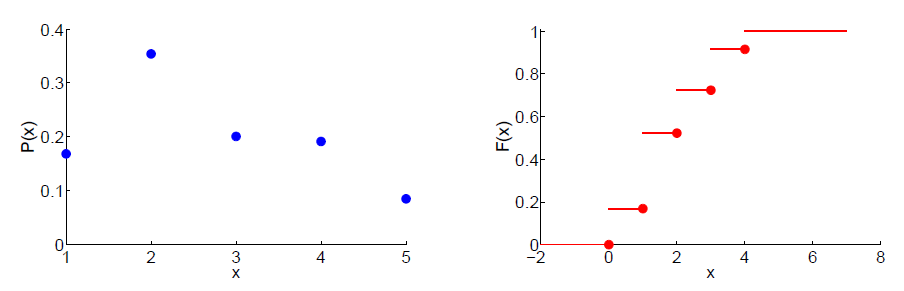
\includegraphics[width=\textwidth]{df1.png}

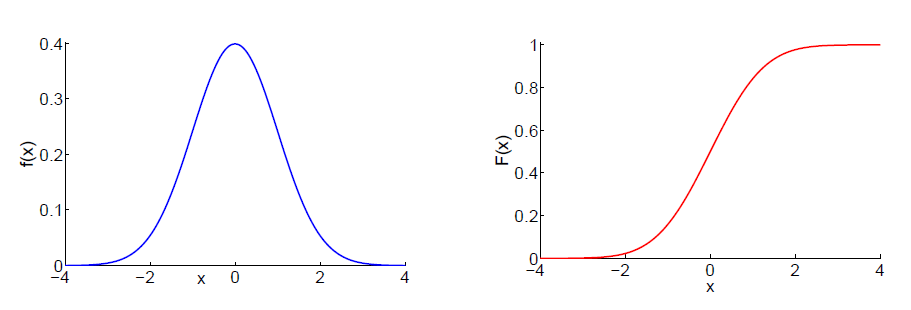
\includegraphics[width=\textwidth]{df2.png}
\end{frame}


\section{Bernoulli scheme}
\begin{frame}
\frametitle{Bernoulli scheme}

\begin{block}{Bernoulli schéma}
Let us consider $n$ independent experiments. The probability that each experiment succeeds is $p$. Then for the variable $X$ which determines the number of successful experiments we get:

\begin{equation}
P(X = k) = \binom{n}{k} p^k (1 - p)^{n-k} 
\end{equation}
\end{block}
\end{frame}

\begin{frame}
\frametitle{12. Exercise}

A student has to finish and exam with 10 questions. Each question has 4 possible answer and only one of them is correct. What is the probability that student who is guessing completely randomly will a) guess at least 5 questions correctly b) at most 5 questions correctly

Solution a)
\begin{itemize}
\item<2-> $P(A) = P(X = 5) + P(X = 6) + P(X = 7) + P(X = 8) + P(X = 9) + P(X = 10)$
\item<3-> $P(X = 5) = \binom{10}{5} 0.25^5 \cdot 0.75^5$
\item<4-> $P(A) = \sum_{k=5}^{10} \binom{10}{k} 0.25^k \cdot 0.75^{10-k}$
\end{itemize}

\end{frame}

\begin{frame}
\frametitle{13. Exercise}

Approximately 75\% of tourists like bryndzové halušky. What is the probability that from 20 tourists a) at least 17 will like halušky b) all of them would like halušky.

\begin{itemize}
\item<2-> $P(A) = P(X = 17) + P(X = 18) + P(X = 19) + P(X = 20)$
\item<3-> $P(X = 20) = \binom{20}{20} 0.75^{20} \cdot 0.25^0 = 0.75^{20}$
\item<4-> $P(A) = \sum_{k=17}^{20} \binom{10}{k} 0.75^k \cdot 0.25^{10-k}$
\end{itemize}
\end{frame}

\section{Distribution parameters}


\begin{frame}
\frametitle{Standard deviation}
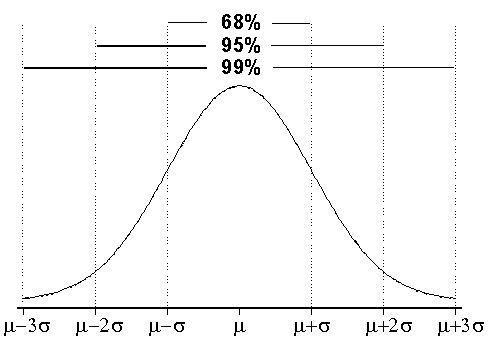
\includegraphics[width = \textwidth]{df3.png}
\end{frame}

\begin{frame}
\frametitle{Approxiamting distribution parameters}

\begin{block}{Sample mean}
$ \overline{X} = \frac{1}{n} \sum_{i=1}^n X_i $
\end{block}

\begin{block}{Sample variance}
$ S^2 = \frac{1}{n-1} \sum_{i=1}^n (X_i - \overline{X})^2 $
\end{block}


\begin{block}{Sample standard deviation}
$S = \sqrt{S^2}$
\end{block}

\begin{block}{Sample covariance}
$S_{XY} = \frac{1}{n-1} \sum_{i=1}^n (X_i - \overline{X})(Y_i - \overline{Y}) $
\end{block}
\end{frame}

\begin{frame}
\frametitle{Approxiamting distribution parameters}

\begin{block}{Confidence intervals}
$P (G_D < \theta < G_H) = 1 - \alpha$
\end{block}

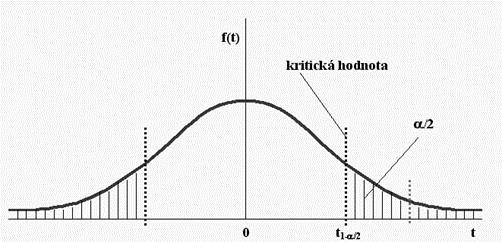
\includegraphics[width=\textwidth]{df4.png}
\end{frame}


\begin{frame}
\frametitle{Approxiamting distribution parameters}

\begin{table}[t]
\begin{tabular}{|l|c|c|c|c|c|}
\hline
$\alpha$     & 0.01   & 0.02   & 0.05   & 0.1    & 0.2   \\ \hline
$u_{\alpha/2}$ & 2.5758 & 2.3263 & 1.9599 & 1.6448 & 1.299 \\ \hline
\end{tabular}
\end{table}
\begin{equation*}
X \sim N(0,1) P(|X| > u_{\alpha/2}) = \alpha
\end{equation*}

\begin{align*}
1 - \alpha &= P(-u_{\alpha/2} < U < u_{\alpha/2}) \\
               &= P(-u_{\alpha/2} < \frac{\overline{X}-\mu}{\sigma} < u_{\alpha/2}) \\
               &= P(\overline{X} - u_{\alpha/2} \cdot \frac{\sigma}{\sqrt{n}} < \mu < \overline{X} + u_{\alpha/2} \cdot \frac{\sigma}{\sqrt{n}})
\end{align*}

\end{frame}


\begin{frame}
\frametitle{Test statistics}

If we know the $\sigma$ value of the original distribution we can use normal distribution:

\begin{equation*}
u = \frac{\overline{X} - \mu_0}{\frac{\sigma}{\sqrt{n}}}
\end{equation*}

If we do not know it and we have $n > 30$ we will use:

\begin{equation*}
u = \frac{\overline{X} - \mu_0}{\frac{S}{\sqrt{n}}}
\end{equation*}

Otherwise we use the Student distribution:

\begin{equation*}
t = \frac{\overline{X} - \mu_0}{\frac{S}{\sqrt{n}}}
\end{equation*}

\end{frame}


\begin{frame}
\frametitle{Test statistics - Matlab}

\begin{block}{Values of $u_{\alpha}$ and $t_{\alpha}$}
For a given confidence interval we can find values of $u_{\alpha}$ and $t_{\alpha}$ from tables. Today we will use Matlab functions.
\end{block}

\begin{block}{norminv}
norminv(alpha) - returns critical value for given alpha for normal distribution
\end{block}

\begin{block}{tinv}
tinv(alpha, n) - returns critical value for given alpha for Students distribution with n degrees of freedom
\end{block}

\begin{block}{Note}
If we desire to obtain a centered confidence interval of 0.95 we need to use $\alpha = 0.975$ (or $[0.025, 0.0975]$).
\end{block}
\end{frame}

\begin{frame}
\frametitle{14. Exercise}

Let us assume that the height of boys of ages 9-10 is distributed normally with unknown mean and standard deviation$\sigma^2=39.112$. We measured a height of 15 boys and calculated the sample mean as 139.13 cm. Determine the 99\% confidence interval for this value.

\begin{itemize}
\item<2-> $n = 15, \sigma  = 6.253, \overline{X} = 139.13$
\item<3-> $1 - \alpha = P(\overline{X} - u_{\alpha/2} \cdot \frac{\sigma}{\sqrt{n}} \leq \mu \leq \overline{X} + u_{\alpha/2} \cdot \frac{\sigma}{\sqrt{n}})$
\item<4-> $139.13 \pm 2.5758 \cdot \frac{6.253}{\sqrt{15}}$
\item<5-> $134.97 \leq \mu \leq 143.28$
\end{itemize}
\end{frame}


\begin{frame}
\frametitle{15. Exercise}
An airliner estimates the average number of travelers. In the last 20 days the average number of travelers was 112 with sample variance of 25. Determine the 95\% confidence interval for the mean of number of travelers $\mu$.

\begin{itemize}
\item<2-> $n = 20, S  = 5, \overline{X} = 112$
\item<3-> $1 - \alpha = P(\overline{X} - t_{\alpha/2, n-1} \cdot \frac{S}{\sqrt{n}} \leq \mu \leq \overline{X} + t_{\alpha/2, n-1} \cdot \frac{S}{\sqrt{n}})$
\item<4-> $112 \pm 2.093 \cdot \frac{5}{\sqrt{20}}$
\item<5-> $109.65 \leq \mu \leq 114.34$
\end{itemize}
\end{frame}


\begin{frame}
\frametitle{16. Exercise}
A random variable $X$ has a normal distribution. The mean and variance are unknown. We measured the following values of $X$: 27, 15, -3, -6, 12, 20, 13, 0, 7, 10. Determine the 95\% confidence interval for the distribution mean.

\begin{itemize}
\item<2-> $n = 10, S  = 10.319, \overline{X} = 9.5$
\item<3-> $1 - \alpha = P(\overline{X} - t_{\alpha/2, n-1} \cdot \frac{S}{\sqrt{n}} \leq \mu \leq \overline{X} + t_{\alpha/2, n-1} \cdot \frac{S}{\sqrt{n}})$
\item<4-> $9.5 \pm 2.262 \cdot \frac{10.319}{\sqrt{10}}$
\item<5-> $2.118 \leq \mu \leq 16.881$
\end{itemize}
\end{frame}

\begin{frame}
\frametitle{17. Exercise}
We picked a sample from a normal distribution with known variance $\sigma^2 = 0.66$. The picked values are: 1.3, 1.8, 1.4, 1.2, 0.9, 1.5, 1.7. Determine the 95\% confidence interval for the mean $\mu$ of the distribution. 

\begin{itemize}
\item<2-> $n = 7, \sigma  = 0.245, \overline{X} = 1.4$
\item<3-> $1 - \alpha = P(\overline{X} - u_{\alpha/2} \cdot \frac{\sigma}{\sqrt{n}} \leq \mu \leq \overline{X} + u_{\alpha/2} \cdot \frac{\sigma}{\sqrt{n}})$
\item<4-> $1.4 \pm 1.9599 \cdot \frac{0.245}{\sqrt{7}}$
\item<5-> $1.218 \leq \mu \leq 1.581$
\end{itemize}
\end{frame}

\begin{frame}
\frametitle{Hypothesis testing - Matlab}

\begin{block}{ztest}
[h, p, ci] = ztest(X, m, sigma, 'Alpha', alpha) - returns a test result for a hypothesis that data in vector X are from a normal distribution with mean of m and standard deviation sigma. h contains 1 if the hypothesis is not confirmed for a given critical value of alpha, otherwise it is zero. ci will contain the confidence interval.
\end{block}

\begin{block}{ttest}
[h, p, ci] = ttest(X, m, 'Alpha', alpha) - returns a test result for a hypothesis that data in vector X are from a normal distribution with mean of m and unknown standard deviation. h contains 1 if the hypothesis is not confirmed for a given critical value of alpha, otherwise it is zero. ci will contain the confidence interval.
\end{block}

\end{frame}

\begin{frame}
\frametitle{18. Exercise}

We claim that bearing made with an automatic lathe have a diameter mean of 10mm. Using a test with critical values $\alpha = 0.05$ test the hypothesis that if we pick 16 random bearings then their mean is 10.3mm for a) $\sigma^2 = 1$ b)$S^2 = 1.21$ 

Solution a)
\begin{itemize}
\item<2-> $n =16, \sigma = 1, \overline{X} = 10.3$
\item<3-> $1 - \alpha = P(\overline{X} - u_{\alpha/2} \cdot \frac{\sigma}{\sqrt{n}} \leq \mu \leq \overline{X} + u_{\alpha/2} \cdot \frac{\sigma}{\sqrt{n}})$
\item<4-> $10.3 \pm 1.9599 \cdot \frac{1}{\sqrt{16}}$
\item<5-> $9.81 \leq \mu \leq 10.789$
\item<5-> We do not reject the hypothesis
\end{itemize}
\end{frame}

\begin{frame}
\frametitle{18. Exercise}

We claim that bearing made with an automatic lathe have a diameter mean of 10mm. Using a test with critical values $\alpha = 0.05$ test the hypothesis that if we pick 16 random bearings then their mean is 10.3mm for a) $\sigma^2 = 1$ b)$S^2 = 1.21$ 

Solution b)
\begin{itemize}
\item<2-> $n =16, S = 1.1, \overline{X} = 10.3$
\item<3-> $1 - \alpha = P(\overline{X} - t_{\alpha/2, n-1} \cdot \frac{S}{\sqrt{n}} \leq \mu \leq \overline{X} + t_{\alpha/2, n-1} \cdot \frac{S}{\sqrt{n}})$
\item<4-> $10.3 \pm 2.131 \cdot \frac{1.1}{\sqrt{16}}$
\item<5-> $9.71 \leq \mu \leq 10.88$
\item<5-> We do not reject the hypothesis
\end{itemize}
\end{frame}







\end{document}